\documentclass[fontsize=11pt]{article}
\usepackage{amsmath}
\usepackage[utf8]{inputenc}
\usepackage[margin=0.75in]{geometry}
\usepackage{graphicx}
\graphicspath{ {graphs/} }

\title{CSC110 Project: Canada's Carbon Emissions Compared To Other Worldwide Nations, Extrapolated To 2050}
\author{Kowan Chan, Howard He, Girish Sujethan, Carson Zhang}
\date{Monday, December 14, 2020}

\begin{document}
    \maketitle

    \section*{Introduction}
    The industrial era came with audacious ideas, but the costly implementations of its incredible innovations have had serious consequences on Earth’s climate. Since the industrial revolution, the global average temperature has increased by more than 1℃. Due to the burning of coal, natural gases, and other fossil fuels, the Earth has been overproducing greenhouse gases. These gases are pivotal to the survival of life on Earth; they insulate the earth by trapping the Sun’s heat within the atmosphere, which maintains livable temperatures for countless species on the planet (Daniel 2). However, there is far too much greenhouse gas being produced today, especially CO$_2$, meaning that too much heat is being trapped and the planet is getting warmer at an alarmingly quick rate.

    Although nations are aware of the dangers of global warming, economic factors are discouraging drastic action. Developing countries like India are relying heavily on fossil fuels to secure financial autonomy, while the economies of developed countries like Canada have been based on industries that rely heavily on fossil fuels. Abandoning fracking and switching to greener policies would have severe economic repercussions for a nation. Since no industry nor government wants to suffer the backlash from such changes, not enough is being done in the present to mitigate global warming. However, institutions are pursuing a path of folly: by 2100, damages related to global warming will be costing \$1.9 trillion annually (Max 3). Even economically, present industry policies will not be viable in the long run.

    If significant change is not made by 2050, the global average temperature will increase by 2℃. This will cause almost 2.7 billion people to be exposed to heat waves every five years. It would also increase sea levels, which could impact a billion people by 2050 (Mode 1). As a country, we must significantly cut down our emissions, or we will see significant consequences in the next thirty years.
    Our research question is \textbf{“in 30 years, how will Canada compare to other countries in carbon emission output?”} It is important to track future emissions overall, but especially domestically where our impact can be most felt. In order to get a relative understanding of a typical country’s carbon emissions in thirty years, we have selected a variety of countries with notably different carbon outputs. By calculating and visualizing information to predict Canada’s future emissions and how they compare to other nations worldwide, we can discern the extent by which we need to change environmental policies today to prevent disaster in the future. Additionally, we will produce a three-dimensional graph, plotting both Canada's GDP per capita and its carbon emissions over the years to contextualize the country's performance. As a first-world country with a large economy, properly assessing Canada's environmental performance means we must also factor in its wealth.


    \section*{Dataset Description}

    All but one of the external datasets used in our project were collected from the website of Knoema, a data technology company. Every dataset is in csv format, each detailing an individual country’s carbon emissions over the years. The seven countries we have selected for this project are Canada, China, Japan, Mexico, Niger, the United Kingdom and the United States of America. All of the datasets can be found within the /datasets folder, with their names listed below:

    Canada$\_$-$\_$CO2$\_$emissions.csv

    China$\_$-$\_$CO2$\_$emissions.csv

    Japan$\_$-$\_$CO2$\_$emissions.csv

    Mexico$\_$-$\_$CO2$\_$emissions.csv

    Niger$\_$-$\_$CO2$\_$emissions.csv

    United$\_$Kingdom$\_$-$\_$CO2$\_$emissions.csv

    United$\_$States$\_$of$\_$America$\_$-$\_$CO2$\_$emissions$\_$2.csv

    Within these csv files, we skipped the first three columns from left to right when collecting data to graph due to their irrelevance to actual data plotting. The name of the country in column 4 is used, and every column afterwards is used to produce separate tuples containing x and y coordinates for the points that we graph.

    Using these datasets, we created our own dataset, a list of individually filtered country datasets, each mapping a country’s name to a tuple containing a list of years and a list of the country’s corresponding carbon emissions over those years. This dataset’s keys are used to label countries on their graphs, and the tuples inside its key-value lists are used to map out the change in carbon emissions of that respective country over time.

    The other external dataset we used was Canada$\_$GDP.csv, a dataset we got from Data Commons. We used both columns in the csv file, the former being a list of years and the latter being a list of those years' corresponding GDPs per capita in Canada.

    \section*{Computational Overview}
    Major Computations:

    main.py uses the get$\_$all function to produce a list of every country's respectively filtered dataset by using storage.append() inside a for loop, whose iterations equal the number of countries inside the input list.

    In order to do so, the get$\_$all uses the extraction.get$\_$data() function on every dataset given by filenames.

    The get$\_$data function in extraction filters a country's carbon emission data into plotting data. The dictionary is developed by using a comprehension which only uses values from 4 to the end of headers; therefore, it avoids the redundant first three columns when creating plotting data.

    To turn (x, y) tuples into graphing information, main.py's convert$\_$all function uses a for loop whose iterations equal the number of country's datasets. By defining a blank dictionary and mutating it with each country's filtered data. The function's maps a country's name to a tuple containing all of that country's years, or "x" values, in one list and its carbon emissions, or "y" values, into another list in order to plot them.

    The values inside the US data are imperial instead of metric: therefore we used the us$\_$conversion function to convert all tonnes values into metric tonnes using a for loop and mutating the carbon emission list.

    To plot the linear graphs, linear$\_$regression.py uses the function simple$\_$linear$\_$regression. First, the function computes mean x and y values by collecting each individually and calculating their sums before dividing them by their number. After calculating b with a for loop, a is calculated by isolation using y = ax + b, using mean x and y for x and y.

    Additionally, to allow the lines some area for error, the function evaluate$\_$line takes the given a, x, and b values along with an acceptable margin of error. If that margin of error is not zero, then the output y = ax + b is added to a random number between -error and error using the function random.uniform(-error, error) and using $\pm$ error as the inputs.

    To get GDP values for the three-dimensional graph visualized in threeD$\_$graph.py, extraction.py uses the get$\_$gdp function. Opening a file given its name, it fills the empty list of GDP values, gdp$\_$so$\_$far, by appending every year's GDP through a while loop which runs when the year whose GDP is being assessed is within the appropriate bounds. Afterwards, since the GDP values are now backwards, another list, reversed$\_$gdp$\_$so$\_$far, is filled by popping every value of gdp$\_$so$\_$far and appending it into reversed$\_$gdp$\_$so$\_$far to flip the GDP values into the desired order.

    To derive information from our graphs for further analysis, we also created a calculations.py file with functions designed to assess veracity of our graphs and to compute information about their slopes.

    The iroc function, short for instantaneous rate of change, is used to derive slopes using a single point on the graph. Taking its dataset and one year from its list as the instant to be calculated, it uses poly$\_$fit to develop the line before returning its slope between two extremely close points. Since we cannot use limits to compute this value, we used 0.001 in place of an infinitesimal value.

    The aroc function, short for average rate of change, can be used to calculate the slope of a graph over a certain set of values. After taking two different years for comparison and a dataset, it produces a graph using poly$\_$fit. Next, it computes the rate of change in the traditional way: by subtracting one year's carbon emissions from another's and dividing by the difference between the two years.

    The rmse$\_$linear$\_$regression and rmse$\_$polynomial$\_$regression are used to calculate just how accurate a graph is. rmse$\_$linear$\_$regression takes a tuple of two lists, one containing all the x-values and the other all the y-values, and first uses poly$\_$fit to produce the graph. Then the function uses a for loop, running for every x-value, which calculates the regression's y-value before subtracting it from the actual y-coordinate at the given x-value and squaring that value. All of these values are added to the aggregator sum$\_$so$\_$far, which is then divided by the number of x-coordinates and squared. The rmse$\_$linear$\_$regression function operates the same way, but uses linear$\_$regression.simple$\_$linear$\_$regression(), inputting the tuple containing an x-value list and y-value list instead of poly$\_$fit.

    To project what Canada's carbon emissions might be like with current trends, we used the polynomial$\_$prediction function. Taking points, a tuple of two lists containing the x-values and y-values of each point, and a country's name as parameters, it projects their emissions by 2021, 2025, and 2050. First, it uses numpy's poly1d function to determine the graph's shape in variable poly$\_$fit. That function takes numpy's polyfit function as a parameter, which takes the x and y values of points as two parameters, and int 5 to indicate the degree. With that information, poly$\_$fit can predict any country's projected emissions in a year like so: poly$\_$fit(year).

    In order to visualize our computations, we imported the new libraries plotly, numpy, and matplotlib. With these new libraries, we were able to take the data we filtered out of the country's datasets and plot it onto various graphs.

    For the linear graphs, we used plotly.graph$\_$objects and imported it as go. After plot$\_$points$\_$and$\_$regression creates its x and y values, we used fig = go.Figure() to produce a blank figure on which we plotted our data. With fig as our object, we used the function update$\_$layout to assign a title, x-axis title, and y-axis title to the graph. Afterwards, we used the add$\_$trace function to input the data, taking the function go.Scatter as a parameter. Scatter function places the given points all over the figure, which is actually added to the graph by add$\_$trace. The add$\_$trace function is used again to add the regressive line, and fig.show() outputs the graph. The graphs are displayed with a toolbar, which allows the visual to be manipulated in several ways, like panning and zooming.

    For the polynomial Canadian graph, we used the numpy and matplotlib's pyplot as external libraries, imported as np and plt respectively. Taking a tuple containing lists of x-values and y-values, points, and the graph's title, it produces a polynomial function. Using the points' two lists as the x and y values, the function uses poly$\_$fit to produce a polynomial graph. Afterwards, it uses xx = np.linspace(1970, 2018, 1000) to collect information to be plotted. The first two parameters are the range of years, and the third is the number of examples generated. Variable xx is placed into the function plot.plot, which plots the graph. plt.title, plt.xlabel, and plt.ylabel are used to label the graph, and plt.axis gives the ranges of the x and y axes, respectively. The actual graph is produced with plt.grid(True) and plt.scatter, and plt.show() visualizes the graph. Just like the linear graphs, this graph is automatically equipped with interactive details, like panning and zooming.

    The three-dimensional graph imports plotly.graph$\_$objects as go in order to visualize itself. Taking lists x and y, containing lists of x-values and y-values of points respectively, as inputs, function call$\_$3d$\_$graph determines variable z by calling the get$\_$gdp function from extraction, using Canada$\_$GDP.csv as the input. Then, the Figure object fig is defined, using x, y, and z as parameters for the parameter function Scatter3d, which plots the values across the graph. fig.update$\_$layout is used to add the graph title, as well as titles for every axis, and fig.show() produces the graph. This graph shares the same interactivity as the others, but it can also be dragged by the cursor to view it from different angles since it is three-dimensional.


    \section*{Interactivity}
    Various aspects of the visualized project can be interacted with. All linear regressions can be controlled with the toolbar at the top of the page in order to zoom in, zoom out, pan, and save the graph. The three-dimensional graph has similar features in its toolbar, but can also be controlled by dragging the cursor around to look at the graph from different angles. Additionally, the graph can zoom in by dragging the cursor downwards, while dragging the cursor upwards zooms out. Canada's polynomial regression also has a toolbar at the bottom that can be used to zoom in on the graph; this is particularly useful because the initial scale makes the graph appear flat. The home button resets the graph, the magnifying glass button allows you to select a select a portion to zoom in on, the printing button allows the graph to be saved, the panning button enables the user to move around the graph by dragging it with the cursor, and the left and right arrows are undo and redo buttons, respectively.

    \section*{Program Instructions}
    Since the latest version of numpy has bugs yet to be completely cleared up, here are instructions to download a previous version of numpy that can properly run our project:

    1. First, find the python38 folder

    Example pathway:
    C:\textbackslash Users \textbackslash girish\textbackslash AppData\textbackslash Local\textbackslash Programs\textbackslash Python\textbackslash Python38\textbackslash Scripts

    2. In the scripts folder, create a new text file and write "cmd" in it, save this file as local.bat to open the windows console

    3. In the console enter ''pip install numpy==1.19.3''

    All of the links where we collected our datasets can be found below:

    https://knoema.com/atlas/Canada/CO2-emissions

    https://knoema.com/atlas/China/CO2-emissions

    https://knoema.com/atlas/Japan/CO2-emissions

    https://knoema.com/atlas/Mexico/CO2-emissions

    https://knoema.com/atlas/Niger/CO2-emissions

    https://knoema.com/atlas/United-Kingdom/CO2-emissions

    https://knoema.com/atlas/United-States-of-America/CO2-emissions

    datacommons.org/tools/timeline\#\&amp;place=country/CAN&amp;

    statsVar=Amount$\_$EconomicActivity$\_$GrossDomesticProduction$\_$Nominal$\_$PerCapita. \\

    However, Knoema requires users to pay for the installation of more than one dataset: therefore, we have compiled all of our datasets at the link below.

    https://mega.nz/file/T8Z3gI4Z#7ew0KmuCqy60hQgdhXK2OcWxpMebLhSZ9QY6ELn8dGo

    The installation of the zipped file from mega.nz provides access to all of our resources, which should be saved in a separate folder called "datasets".

    \section*{Project Changes}
    The primary difference between our project proposal and our ultimate project is the inclusion of Canada's GDP per capita in a three-dimensional graph that also plots Canada's annual carbon emissions. Other countries we assessed, such as the United States, have much bigger economies and industries than Canada, while other countries like Niger are much less developed than Canada. In order to properly evaluate Canada's carbon emissions, we felt that contextualizing the country's emissions with its GDP per capita would be an effective way of putting its carbon production into context.

    The other difference is the datasets that we chose. We replaced India with Niger, because we felt that the country's environmental impacts were much more distinguishable from Canada's than India's. Additionally, to better compare Canada with its peers, we also added the United States and United Kingdom because of their similarities to our own country.

    \section*{Discussion}
    The results derived from the graphs produced illuminate a great deal about our research question, \textbf{“in 30 years, how will Canada compare to other countries in carbon emission output?”} First of all, we can see how Canada is faring compared to other countries today just by looking at the slopes of the following linear graphs!

    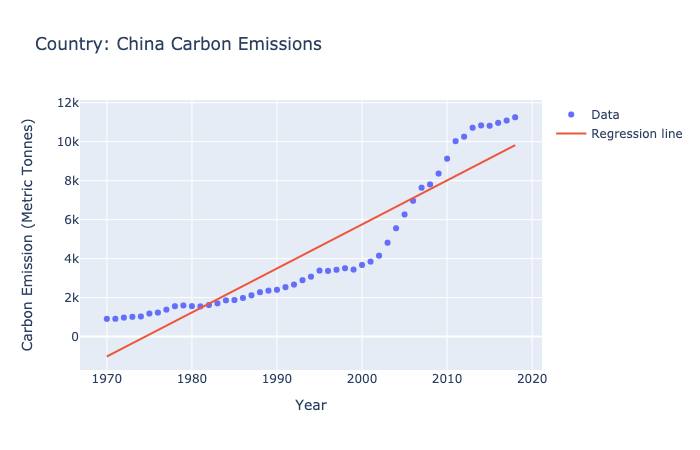
\includegraphics[scale=0.75]{china_linear.png}
    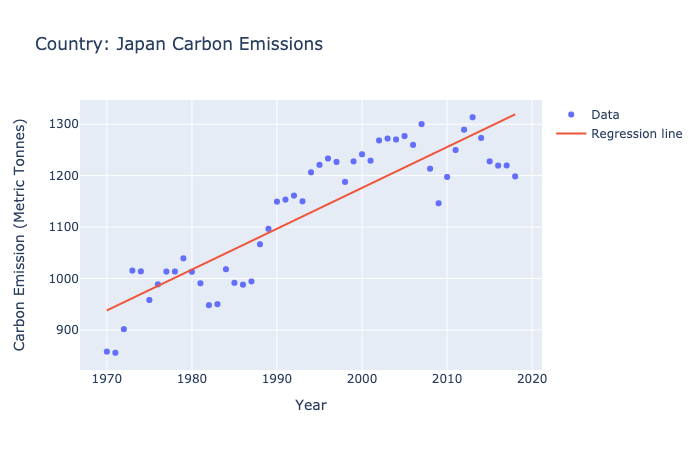
\includegraphics[scale=0.75]{japan_linear.png}
    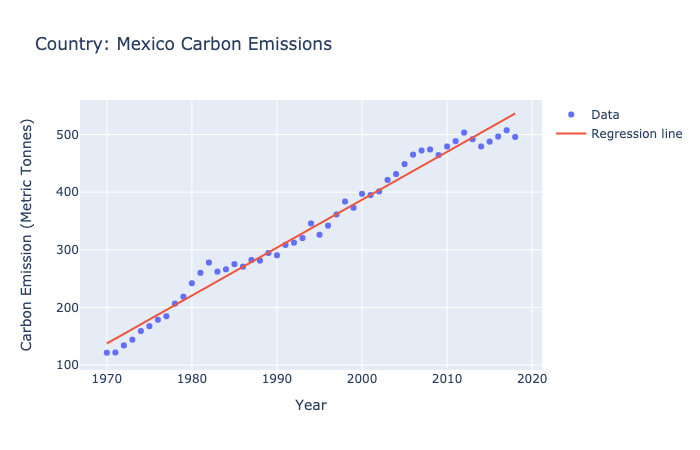
\includegraphics[scale=0.75]{mexico_linear.png}
    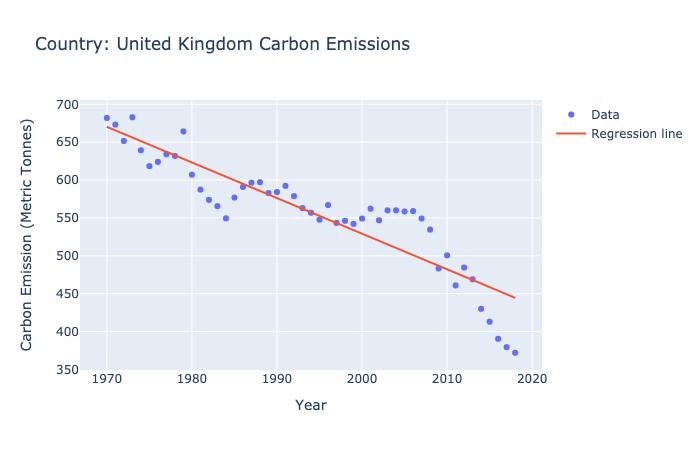
\includegraphics[scale=0.75]{uk_linear.png}
    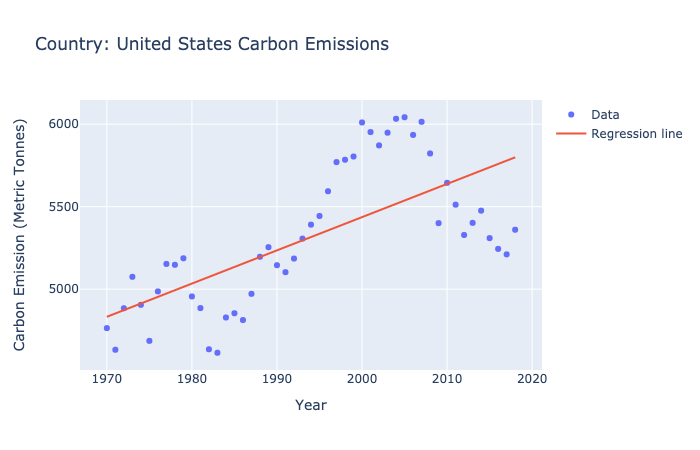
\includegraphics[scale=0.75]{us_linear.png}
    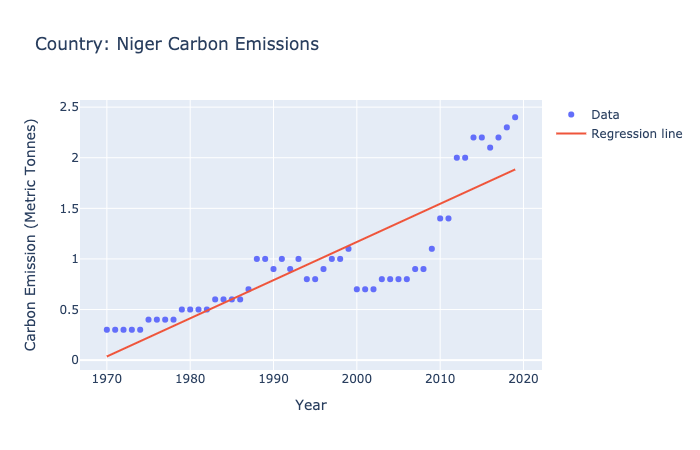
\includegraphics[scale=0.75]{niger_linear.png}
    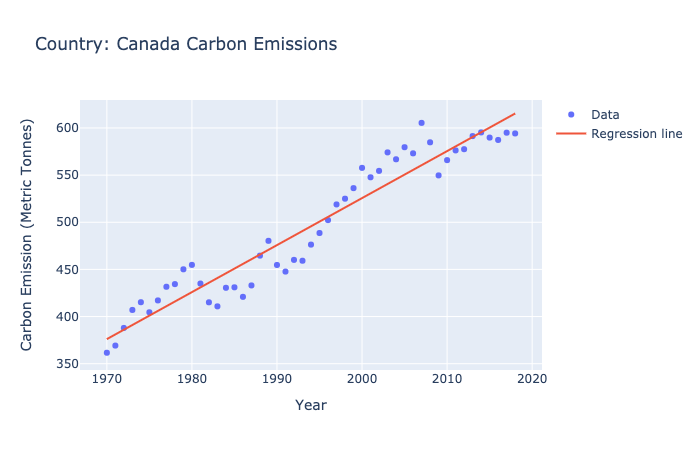
\includegraphics[scale=0.75]{canada_linear.png}

    A more direct comparison can be drawn between Canada and the outside world by comparing the above graph of Canada with a graph combining all the points of the other countries into one graph. Canada's graph appears much steeper than the global graph, which suggests Canada's environmental efforts are not going very well.

    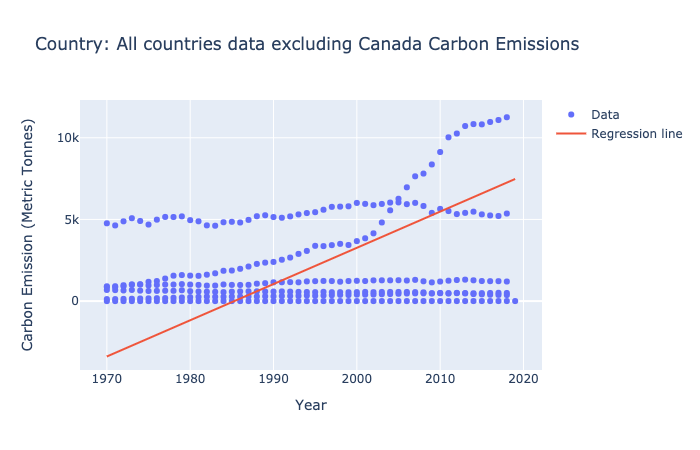
\includegraphics[scale=0.6]{global_linear.png}

    Additionally, we can rely on the instantaneous and average rate of change functions in calculations.py, iroc and aroc, to find concrete numbers regarding Canada and other nations' change in carbon emissions over the years. Since much more effort has been made in recent years to address climate issues, we evaluated the average rate of change experienced in each country between 2000 and 2018 to see how they were performing in the 21st century.

    From the lowest slope to the highest slope, the countries are: US: -30.94 tonnes/year, UK: -11.33 tonnes/year, Japan: -0.30 tonnes/year, Niger: 0.09 tonnes/year, Canada: 3.25 tonnes/year, Mexico: 5.45 tonnes/year, China: 388.29 tonnes/year

    Just like in the graphs, our data shows that Canada is clearly underperforming when it comes to environmental change. The same is true when evaluating instantaneous rates of change in 2018.

    From lowest slope to highest, the countries are: China: -343.75 tonnes/year, UK: -24.60 tonnes/year, Mexico: -9.16 tonnes/year, Niger: 0.09 tonnes/year, Canada: 10.01 tonnes/year, Japan: 20.26 tonnes/year, US: 101.56 tonnes/year

    Especially since the United States' extremely high tangent is due to a single spike between 2017 and 2018 after two drastically declining decades, it is evident from our computations that Canada is not doing as much as other countries to reduce its carbon emissions.

    In order to look at how Canada, and other countries, might do in the future, we used polynomial regression to get a potentially more accurate view of our country's future emissions.

    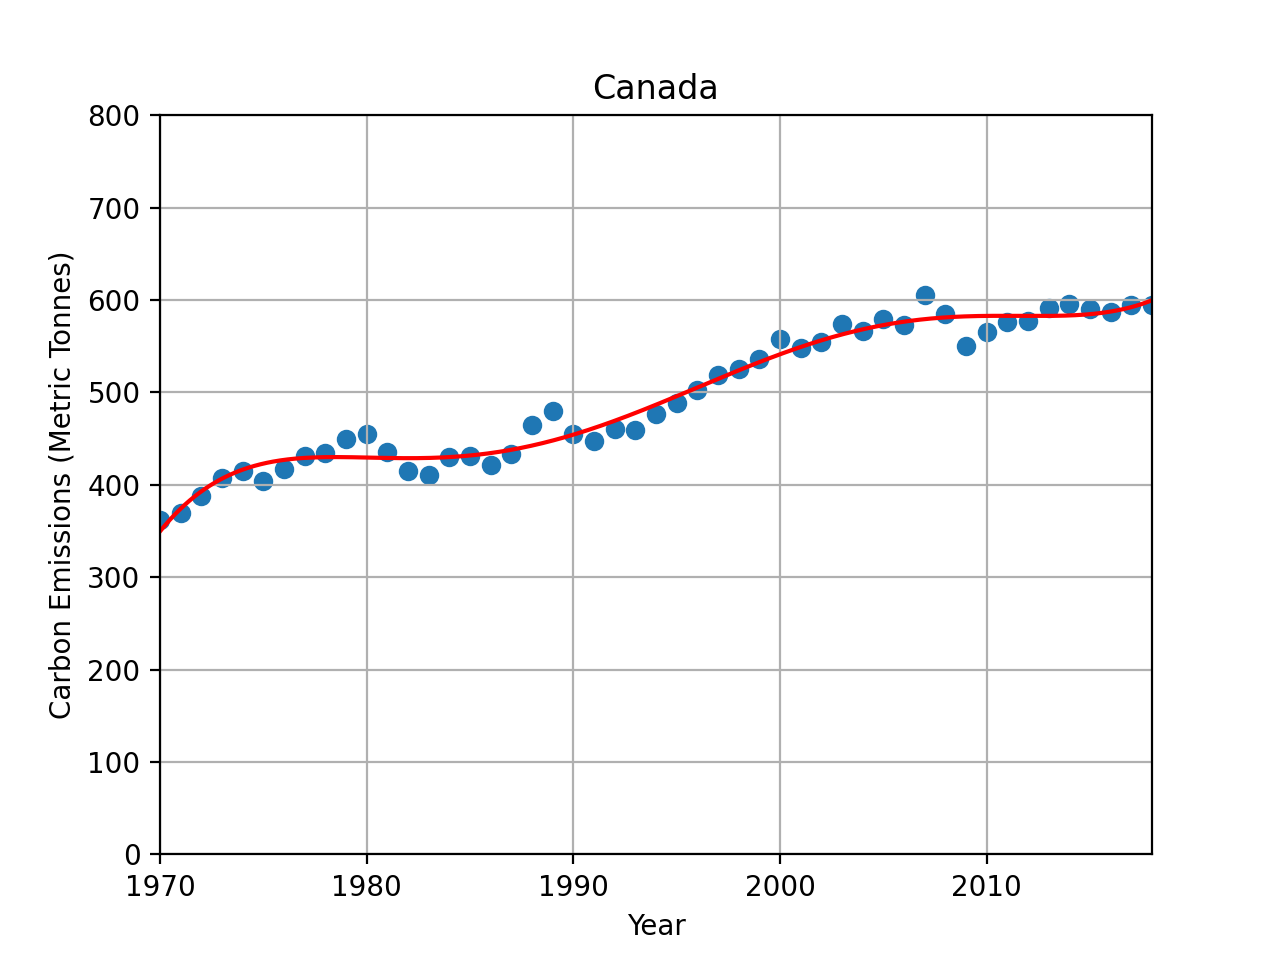
\includegraphics[scale = 0.75]{canada_polynomial.png}

    This polynomial graph has positive implications for Canada as the curve has considerably flattered over the past few decades, but the notable uptick at the end of the graph means that our projection will suggest that Canada's emissions will get exponentially worse by 2050. By using the polynomial$\_$prediction function from poly$\_$regression.py, we can extrapolate countries' carbon emissions from 2021 to 2025 to 2050. Note: the values projected follow the slopes, and so can be negative. In increasing order by 2050, the countries are:

    China

    2021: 8856.26 tonnes, 2025: 848.11 tonnes, 2050: -478374.10 tonnes


    Mexico

    2021: 442.78 tonnes, 2025: 317.39 tonnes, 2050: -4844.28 tonnes

    UK

    2021: 274.26 tonnes, 2025: 140.34 tonnes, 2050: -836.26 tonnes


    Niger

    2021: 2.56 tonnes, 2025: 2.10 tonnes, 2050: -80.79 tonnes

    Japan

    2021: 1355.87 tonnes, 2025: 1733.76 tonnes, 2050: 26537.00 tonnes

    Canada

    2021: 645.42 tonnes, 2025: 797.19 tonnes, 2050: 11503.41 tonnes

    US

    2021: 5939.00 tonnes, 2025: 8246.73 tonnes, 2050: 171889.58 tonnes

    Leading Japan by over four times in this projection by 2050, and given all the other evidence collected, our project suggests that Canada will continue to be one of the worse countries around the world in terms of carbon emissions by 2050.

    One of the limitations we had with plotly was somewhat of a technical difficulty. The library that we used, plotly, was difficult to understand at first so we never really developed a more advanced set of graphs. What we would have liked to do is put all the graphs on a single browser page so that you would not need to click on different pages. Comparing them when they all existed on the same graph would be much easier. Although we could not due to time restraints and our lack of mastery, having all graphs on a single page that could also rotate between different graphs would have been nice. While this is more of a quality of life improvement regarding the library we used, it was a limitation nonetheless.

    Another limitation we encountered was data limitation. The data we found exists as separate files for each country, meaning that our program must do the same collecting and processing of data for each file. What we would have liked to have is one big file with all of the data for each country on it, but no such file existed. The data we obtained was also limited to the range of years spanning from 1970 to 2018, meaning that we are missing a substantial part of the 20th century as well as the most recent years of data. This limits the accuracy of our program since it has less data to average out.

    While the polynomial graph and the projected carbon emissions were handy, the trouble with them was that they failed to account for sudden, incidental spikes in the data. For instance, while Canada has considerably flattened the curve of carbon emission, the graph and projection suggest that emissions will skyrocket by 2050 because of a notable uptick near the end of the 2010s.

    One of the largest and most obvious steps for improvement is to increase the amount of data we collect and process. This means that carbon emission information about the selected countries should span before the 1970s and after 2018. With a larger domain of data, we can have more accuracy in our data. Another way to increase the amount of data we process is to get more countries involved. This means gathering data from countries that we have not analyzed yet. By doing this, we widen the scope of comparison when we look at Canada’s standing and therefore have a better understanding of how Canada compares to other countries. Additionally, using plotly to shrink the number of graphs by compiling many into one would be an extreme improvement.

    Although the polynomial graph did show Canada has been impressively reducing its reliance on fossil fuels in recent years, our graphs and calculations show that Canada still has a long way to go. While we did produce a three-dimensional graph including GDP per capita to contextualize and somewhat explain Canada's reliance on fossil fuels, our data shows that both countries wealthier and poorer than Canada are outperforming our country's efforts to become greener. The US, with similar living standards to Canada, has a flatter positive slope on the linear graphs, while the UK has a significantly negative slope. In order to secure a stable future, economically and environmentally, Canada needs to speed up its greening process to match other countries around the world.
    \section*{References}


    \begin{center}
        Works Cited
    \end{center}
    “3D Scatter Plots.” \textit{Plotly},, 2016, plotly.com/python/3d-scatter-plots/. \\
    \newline
    Bailey, Daniel. “FAQ: What Is the Greenhouse Effect?” \textit{NASA}, NASA, 2020,
    \newline

    climate.nasa.gov/faq/19/what-is-the-greenhouse-effect/. \\
    \newline
    “Canada's GDP per Capita 1960–2018.” \textit{Data Commons} , 2018, datacommons.org/tools/timeline\#\&amp;place=country/ \\

    CAN&amp;statsVar=Amount$\_$EconomicActivity$\_$GrossDomesticProduction$\_$Nominal$\_$PerCapita. \\
    \newline
    Knoema. “Canada CO2 Emissions, 1970-2019.” \textit{Knoema}, 2018, knoema.com/atlas/Canada/CO2-emissions.  \\
    \newline
    Knoema. “China CO2 Emissions, 1970-2019.” \textit{Knoema}, 2018, knoema.com/atlas/China/CO2-emissions. \\
    \newline
    Knoema. “Japan CO2 Emissions, 1970-2019.” \textit{Knoema}, 2018, knoema.com/atlas/Japan/CO2-emissions.  \\
    \newline
    Knoema. “Mexico CO2 Emissions, 1970-2019.” \textit{Knoema}, 2018, knoema.com/atlas/Mexico/CO2-emissions.  \\
    \newline
    Knoema. “Niger CO2 Emissions, 1970-2019.” \textit{Knoema}, 2018, knoema.com/atlas/Niger/CO2-emissions.  \\
    \newline
    Knoema. “United Kingdom CO2 Emissions, 1970-2019.” \textit{Knoema}, 2018,   \\

    \newline

    knoema.com/atlas/United-Kingdom/CO2-emissions. \\
    \newline
    Knoema. “United States of America CO2 Emissions, 1970-2018.” \textit{Knoema}, 2018, \\

    \newline
    knoema.com/atlas/United-States-of-America/CO2-emissions. \\
    \newline
    “Machine Learning - Polynomial Regression.” \textit{Python Machine Learning Polynomial Regression}, 2016, \\

    www.w3schools.com/python/python$\_$ml$\_$polynomial$\_$regression.asp. \\
    \newline
    Mode, Hannah. “Our Planet Is Warming. Here's What's at Stake If We Don't Act Now.” \textit{WWF, World Wildlife} \\

    \newline
    \textit{Fund}, 2020, www.worldwildlife.org/stories/our-planet-is-warming-here-s-what-s-at-stake-if-we-don-t-act-now.\\
    \newline
    “Plotly Python Graphing Library.” \textit{Plotly}, 2020, plotly.com/python/. \\
    \newline
    Roser, Max. “Future Greenhouse Gas Emissions.” \textit{Our World in Data}, 2018, ourworldindata.org/future-emissions.\\
    \newline
    Statistics How To. “RMSE: Root Mean Square Error.” \textit{Statistics How To}, 6 July 2020, \\

    \newline
    www.statisticshowto.com/probability-and-statistics/regression-analysis/rmse-root-mean-square-error/.
% NOTE: LaTeX does have a built-in way of generating references automatically,
% but it's a bit tricky to use so we STRONGLY recommend writing your references
% manually, using a standard academic format like APA or MLA.
% (E.g., https://owl.purdue.edu/owl/research_and_citation/apa_style/apa_formatting_and_style_guide/general_format.html)

\end{document}

